% Source p.1 (965). P is a schematic position on DC.
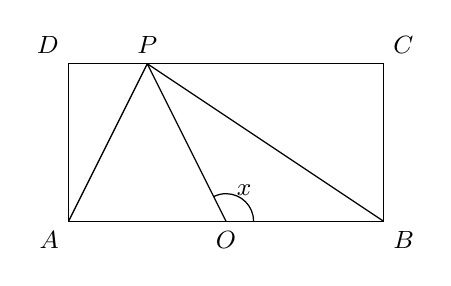
\begin{tikzpicture}[line width=.45pt,font=\small]
  \coordinate (A) at (0,0); \coordinate (B) at (4,0);
  \coordinate (C) at (4,2); \coordinate (D) at (0,2);
  \coordinate (O) at (2,0); \coordinate (P) at (1,2);
  \draw (A)--(B)--(C)--(D)--cycle;
  \draw (A)--(P)--(B) (P)--(O);
  \draw (2.35,0) arc[start angle=0,end angle=116.565,radius=.35];
  \node at (2.23,.39) {$x$};
  \node[below left] at (A) {$A$}; \node[below right] at (B) {$B$};
  \node[above right] at (C) {$C$}; \node[above left] at (D) {$D$};
  \node[below] at (O) {$O$}; \node[above] at (P) {$P$};
\end{tikzpicture}
